\documentclass[10pt]{article}
\usepackage[polish]{babel}
\usepackage[utf8]{inputenc}
\usepackage[T1]{fontenc}
\usepackage{amsmath}
\usepackage{amsfonts}
\usepackage{amssymb}
\usepackage[version=4]{mhchem}
\usepackage{stmaryrd}
\usepackage{graphicx}
\usepackage[export]{adjustbox}
\graphicspath{ {./images/} }
\usepackage{hyperref}
\hypersetup{colorlinks=true, linkcolor=blue, filecolor=magenta, urlcolor=cyan,}
\urlstyle{same}

\title{Zadania - etap I (kl. I i II gimnazjum) }

\author{}
\date{}


\begin{document}
\maketitle
CENTRUM NAUCZANIA MATEMATYKI\\
I KSZTALCENIA NA ODLEGŁOSĆ

Zadanie 1. Oblicz wartość ułamka: \(\frac{36 \cdot 18^{n}-8 \cdot 2^{n-4} \cdot 9^{n}-3^{n+1} \cdot 6^{n+1}}{18^{n-1}}\), gdzie \(n\) jest dowolną liczba naturalną.

Zadanie 2. Liczby \(a\) i \(b\) spełniają równanie:

\[
(a-b)^{2}+(a+b-4)^{2}=0 .
\]

Wyznacz wartość iloczynu \(a^{2}(b+1)\).\\
Zadanie 3. Wykaż, że liczba: \(3^{1}+3^{2}+3^{3}+\ldots+3^{998}+3^{999}\) jest podzielna przez 13 .\\
Zadanie 4. Dany jest kwadrat \(A B C D\) o boku długości \(a\). Punkty \(M\) i \(N\) leżą na odcinku łączącym środki boków \(B C\) i \(A D\) tak, że pole czworokąta \(A N C M\) jest \(\frac{1}{3}\) pola kwadratu \(A B C D\). Wykaż, że długość odcinka \(M N\) wynosi \(\frac{2}{3} a\).\\
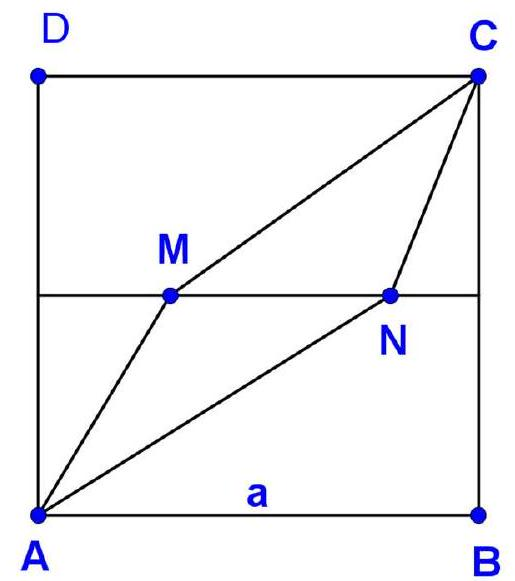
\includegraphics[max width=\textwidth, center]{2024_11_21_e97811247d06ebb2c513g-1}

Zadanie 5. lle wynosi różnica:

\[
\left(1^{2}+2^{2}+3^{2}+\ldots+2016^{2}\right)-(1 \cdot 3+2 \cdot 4+3 \cdot 5+\ldots+2015 \cdot 2017) ?
\]

Wskazówka: Zastosuj wzór: \(a^{2}-b^{2}=(a-b)(a+b)\).\\
imię i nazwisko uczestnika

CENTRUM NAUCZANIA MATEMATYKI\\
I KSZTALCENIA NA ODLEGLOŚ\\
\(\qquad\)

\section*{ZAŁACZNIK DO KARTY UCZESTNIKA KONKURSU „OD SZKOLNIAKA DO ŻAKA"}
\section*{Oświadczenie}
Niniejszym oświadczam, że jako uczestnik konkursu „Od szkolniaka do żaka" zorganizowanego przez Centrum Nauczania Matematyki i Kształcenia na Odległość Politechniki Gdańskiej, wyrażam zgodę na przetwarzanie moich danych osobowych w zakresie niezbędnym dla potrzeb niniejszego konkursu.

Przyjmuję do wiadomości, że moje dane osobowe będą wykorzystane zgodnie z ustawą z dnia 29 sierpnia 1997 r. o ochronie danych osobowych (Dz.U. 1997 nr 133 poz. 883) dla celów przeprowadzenia w/w konkursu.

Jednocześnie oświadczam, że zostałem poinformowany o tym, że:

\begin{itemize}
  \item Administratorem danych osobowych konkursu jest: Politechnika Gdańska z siedzibą przy ul. Gabriela Narutowicza 11/12; 80-233 Gdańsk
  \item Przysługuje mi prawo do wglądu do moich danych i żądania ich poprawienia.
  \item Dane będą przetwarzane dla realizacji konkursu.
  \item Podanie danych jest dobrowolne.
  \item Nie przewiduje się przekazywania danych.
\end{itemize}

Wyrażam zgodę na uczestnictwo mojego dziecka w konkursie „Od szkolniaka do żaka"

Data \(\qquad\) r.\\
(podpis rodzica lub opiekuna prawnego ucznia)

Akceptuję i wyrażam zgodę na postanowienia regulaminu konkursu „Od szkolniaka do żaka" zamieszczonego na stronie internetowej konkursu: \href{http://pg.edu.pl/kursy-z-matematyki/o-konkursie}{http://pg.edu.pl/kursy-z-matematyki/o-konkursie}

Data \(\qquad\) r.


\end{document}